\documentclass[aspectratio=169]{beamer}
% \pdfpagewidth=1920bp
% \pdfpageheight=1080bp
\setbeamertemplate{navigation symbols}{}
\setbeamertemplate{headline}{} % No headline
\setbeamertemplate{bibliography item}{} % No icons
\usepackage{tikz}
\usepackage{hyperref}
\usepackage{booktabs}
\usepackage{tikz}
\usepackage{multirow}
\usetikzlibrary{positioning,calc}

\graphicspath{{../figs/}}

% --- Hyperref setup: make citation links blue ---
\hypersetup{
  colorlinks=true,
  linkcolor=blue,
  citecolor=blue,
  urlcolor=blue
}


% --- Biblatex setup ---
\usepackage[
  backend=biber,
  style=keynote,
  citestyle=keynote,
  maxbibnames=1,
  uniquename=false,
  sorting=none
]{biblatex}
\addbibresource{references.bib}
% --- Helper: left-bottom reference box ---
\renewcommand*{\bibfont}{\fontsize{5}{6}\selectfont}
\newcommand{\bottomleftrefs}{%
  \begin{tikzpicture}[remember picture,overlay]
    \node[anchor=south west, xshift=1pt, yshift=1pt] at (current page.south west) {%
      \parbox{0.9\linewidth}{
        \setlength{\bibitemsep}{0pt plus 0.3ex}
        \printbibliography[heading=none]
      }
    };
  \end{tikzpicture}%
}

% --- Custom footline with annotated adjustments ---
\setbeamertemplate{footline}{%
  \leavevmode%
  % ----- LEFT: citation area -----
  \begin{minipage}[b]{0.70\paperwidth}
    \vspace{0.2em}
    {%
      % Set font size and type for the citation area
      \fontsize{8}{10}\selectfont % (8pt, 10pt line spacing)
      \textsf{ % Sans-serif font for references
        \ifdefined\slidebib
          \slidebib
        \fi
      }
    }
  \end{minipage}%
  \hfill
  % ----- RIGHT: copyright area -----
  \begin{minipage}[b]{0.28\paperwidth}
    \vspace{0.2em}
    \raggedleft
    {%
      % Set font size and type for copyright
      \fontsize{9}{11}\selectfont % (9pt, 11pt line spacing)
      \textrm{ % Serif font for copyright
        \textcopyright~2025 Sakura
      }
    }
  \end{minipage}%
}

% Helper macro: define per-slide bibliography (reset on every slide)
\newcommand{\slidebib}{}

%--- Metadata ---
\title[]{Diffusion Models for Image Generation in Remote Sensing}
\subtitle{GISLab Short-Term Course 2025 Summer}
\author[Sakura]{\href{https://bili-sakura.github.io/}{Zhenyuan Chen}}
\institute[ZJU]{School of Earth Science, Zhejiang University}
\date{June 25, 2025\\\small\href{mailto:bili_sakura@zju.edu.cn}{bili\_sakura@zju.edu.cn}}

\begin{document}

%--- Cover slide ---
\begin{frame}[plain]
  \begin{tikzpicture}[remember picture,overlay]
    \node[at=(current page.center),opacity=0.4] {\includegraphics[width=\paperwidth,height=\paperheight,keepaspectratio]{landscape.png}};
  \end{tikzpicture}
  \centering
  % \vspace{2.5em}
  {\usebeamerfont{title}\usebeamercolor[fg]{title}\inserttitle\par}
  \vspace{0.5em}
  {\usebeamerfont{subtitle}\usebeamercolor[fg]{subtitle}\insertsubtitle\par}
  \vspace{1.5em}
  % 
\includegraphics[width=0.22\linewidth,clip,keepaspectratio]{profile_new.jpeg}
  % \vspace{1.2em}
  
  {\usebeamerfont{author}\usebeamercolor[fg]{author}\insertauthor\par}
  {\usebeamerfont{institute}\usebeamercolor[fg]{institute}\insertinstitute\par}
  % \vspace{1em}
  {\usebeamerfont{date}\usebeamercolor[fg]{date}\insertdate\par}
  % Add left bottom image sourcev
  \vspace{3em}
  \tiny Image Source:~\cite{CVPR2023Tutorial}.
  \bottomleftrefs
\end{frame}

%--- Cover slide will be handled by \titlepage in keynote.tex ---

%--- Slide 1: Outline ---
\begin{refsection}
\begin{frame}{Outline}
  \begin{itemize}
    \item Introduction
    \item Background: Generative Models
    \item Preliminaries: Diffusion Models
    \item Applications in Remote Sensing
    \item Evaluation of Synthetic Data
    \item Project Assignment
    \item Q\&A
  \end{itemize}
\end{frame}
\end{refsection}

\begin{refsection}
\begin{frame}{Generative Modeling}
  \begin{figure}
    \centering
    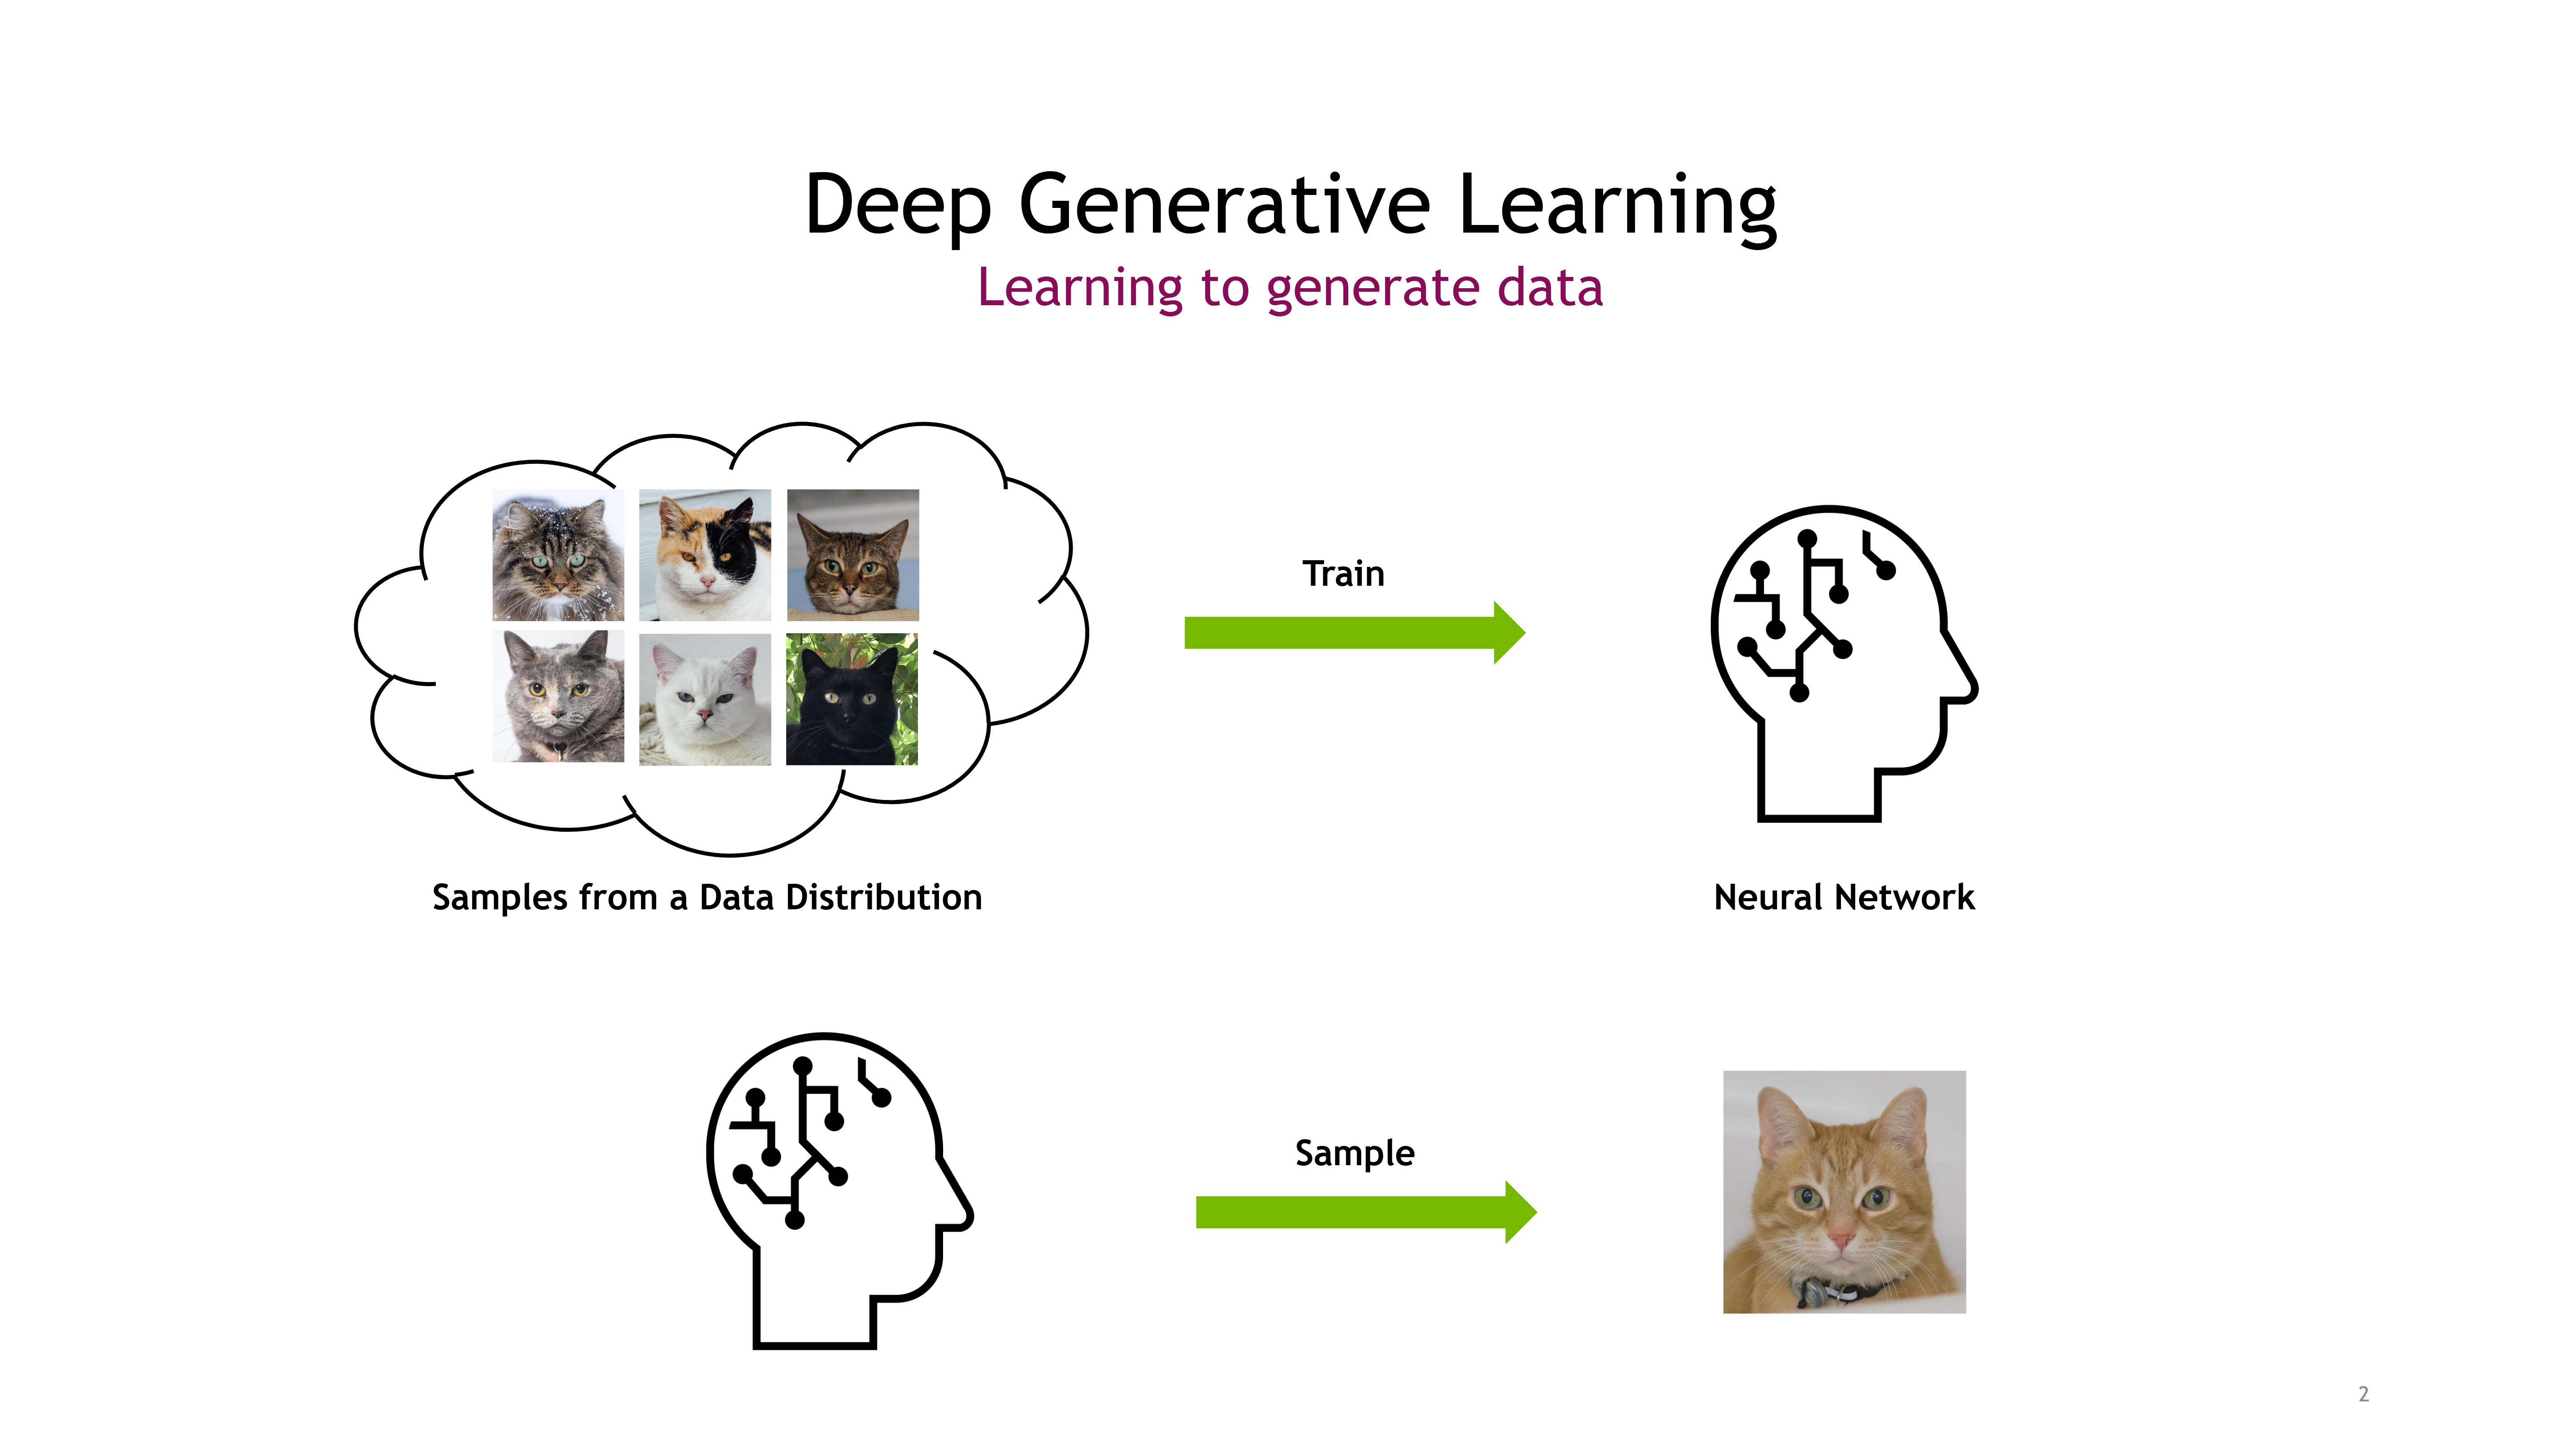
\includegraphics[width=0.8\linewidth]{figs/learning_to_generate_data.png}
    \caption{\scriptsize Illustration of generative modeling~\parencite{CVPR2023Tutorial}.}
  \end{figure}
  \bottomleftrefs
\end{frame}
\end{refsection}

% --- Slide 2: Timeline of Generative Models ---
% \begin{refsection}
% \begin{frame}{Timeline of Generative Models}
%   \begin{figure}
%     \centering
%     % Timeline with time scale corresponding to year
%     \begin{tikzpicture}[x=1.6cm, y=1cm] % Increased x to enlarge the gap
%       % Define years and their positions
%       \def\yVAE{2013}
%       \def\yGAN{2014}
%       \def\yDiff{2015}
%       \def\yDDPM{2020}
%       % Compute min and max year for axis
%       \def\yMin{2013}
%       \def\yMax{2020}
%       % Timeline line
%       \draw[thick] (0,0) -- ({\yMax-\yMin},0);

%       % Draw year ticks
%       \foreach \y in {2013,2014,2015,2016,2017,2018,2019,2020} {
%         \node[below=8pt] at ({\y-\yMin},0) {\scriptsize \y};
%       }

%       % Events
%       \draw[fill=blue!30] ({\yVAE-\yMin},0) circle (2.5mm);
%       \node[above=8pt,align=center,text width=2.8cm] at ({\yVAE-\yMin},0) {\scriptsize VAE\\{\tiny\parencite{kingma2013auto}}};

%       \draw[fill=blue!30] ({\yGAN-\yMin},0) circle (2.5mm);
%       \node[above=8pt,align=center,text width=2.8cm] at ({\yGAN-\yMin},0) {\scriptsize GAN\\{\tiny\parencite{goodfellow2014generative}}};

%       \draw[fill=blue!30] ({\yDiff-\yMin},0) circle (2.5mm);
%       \node[above=8pt,align=center,text width=2.8cm] at ({\yDiff-\yMin},0) {\scriptsize Diffusion\\{\tiny\parencite{sohl2015deep}}};

%       \draw[fill=blue!30] ({\yDDPM-\yMin},0) circle (2.5mm);
%       \node[above=8pt,align=center,text width=2.8cm] at ({\yDDPM-\yMin},0) {\scriptsize DDPM\\{\tiny\parencite{ho2020denoising}}};
%     \end{tikzpicture}
%     \caption{\scriptsize Key milestones in deep generative models.}
%   \end{figure}
%   \bottomleftrefs
% \end{frame}
% \end{refsection}

\begin{refsection}
\begin{frame}{}
  \begin{figure}
    \centering
    \includegraphics[width=0.9\linewidth]{figs/landscape.png}
    \caption{\scriptsize Image Derived from~\parencite{CVPR2023Tutorial}.}
  \end{figure}
  \bottomleftrefs
\end{frame}
\end{refsection}


%--- Slide 3a: Variational Autoencoder (VAE) ---
% \begin{refsection}
% \begin{frame}{Background: Variational Autoencoder (VAE)}
%   \begin{columns}[t]
%     \begin{column}{0.55\textwidth}
%       \begin{itemize}
%         \item \textbf{VAE} is a probabilistic generative model~\parencite{kingma2013auto}.
%         \item Learns to encode data into a latent space and decode back to data.
%         \item Enables smooth interpolation and sampling.
%       \end{itemize}
%       \vspace{0.8em}
%       VAEs introduced a principled approach to generative modeling with latent variables.
%     \end{column}
%     \begin{column}{0.35\textwidth}
%       \begin{figure}
%         \centering
%         \fbox{%
%           \parbox[c][0.16\textheight][c]{\linewidth}{%
%             \centering VAE Schematic
%           }
%         }
%         \caption*{\scriptsize Encoder-decoder structure of VAE.}
%       \end{figure}
%     \end{column}
%   \end{columns}
%   \bottomleftrefs
% \end{frame}
% \end{refsection}

%--- Slide 3b: Generative Adversarial Network (GAN) ---
% \begin{refsection}
% \begin{frame}{Background: Generative Adversarial Network (GAN)}
%   \begin{columns}[t]
%     \begin{column}{0.55\textwidth}
%       \begin{itemize}
%         \item \textbf{GAN} consists of a generator and a discriminator~\parencite{goodfellow2014generative}.
%         \item Trains via adversarial game: generator tries to fool the discriminator.
%         \item Produces highly realistic images.
%       \end{itemize}
%       \vspace{0.8em}
%       GANs revolutionized image synthesis with adversarial training.
%     \end{column}
%     \begin{column}{0.35\textwidth}
%       \begin{figure}
%         \centering
%         \fbox{%
%           \parbox[c][0.16\textheight][c]{\linewidth}{%
%             \centering GAN Schematic
%           }
%         }
%         \caption*{\scriptsize Generator vs. discriminator in GAN.}
%       \end{figure}
%     \end{column}
%   \end{columns}
%   \bottomleftrefs
% \end{frame}
% \end{refsection}

%--- Slide 3c: Diffusion Models ---
\begin{refsection}
\begin{frame}{Background: Diffusion Models}
  \begin{columns}[t]
    \begin{column}{0.55\textwidth}
      \begin{itemize}
        \item \textbf{Diffusion models} generate data by iterative denoising~\parencite{sohl2015deep,ho2020denoising}.
        \item Add noise to data and learn to reverse the process.
        \item Achieve state-of-the-art image quality and diversity.
      \end{itemize}
      \vspace{0.8em}
      Diffusion models are the current frontier in generative modeling.
    \end{column}
    \begin{column}{0.35\textwidth}
      \begin{figure}
        \centering
        \fbox{%
          \parbox[c][0.16\textheight][c]{\linewidth}{%
            \centering Diffusion Schematic
          }
        }
        \caption*{\scriptsize Stepwise denoising in diffusion models.}
      \end{figure}
    \end{column}
  \end{columns}
  \bottomleftrefs
\end{frame}
\end{refsection}

%--- Slide 4: Preliminaries of Diffusion Models ---
\begin{refsection}
\begin{frame}{Preliminaries: Diffusion Models in Image Synthesis}
  \begin{columns}[t]
    \begin{column}{0.6\textwidth}
      \begin{itemize}
        \item Diffusion models generate images by iterative denoising~\parencite{ho2020denoising}.
        \item High fidelity, diverse image generation.
        \item Now state-of-the-art for many generative tasks.
      \end{itemize}
    \end{column}
    \begin{column}{0.3\textwidth}
      \begin{figure}
        \centering
        \fbox{%
          \parbox[c][0.14\textheight][c]{\linewidth}{%
            \centering Diffusion steps visual
          }
        }
        \caption[]{\scriptsize Stepwise denoising in diffusion models.}
      \end{figure}
    \end{column}
  \end{columns}
  \bottomleftrefs
\end{frame}
\end{refsection}

%--- Slide 5: Application in Remote Sensing: DiffusionSat, CRS-Diff, Text2Earth ---
\begin{refsection}
\begin{frame}{Applications: Generative Models for Remote Sensing}
  \begin{itemize}
    \item \textbf{CRS-Diff}: Controllable remote sensing image generation~\parencite{tang2024crsdiff}
    \item \textbf{DiffusionSat}: Large-scale remote sensing text-to-image generation~\parencite{diffusionset2024}
    \item \textbf{Text2Earth}: Foundation model for text-driven Earth observation~\parencite{text2earth2025}
  \end{itemize}
  \begin{figure}
    \centering
    \fbox{%
      \parbox[c][0.12\textheight][c]{0.7\linewidth}{%
        \centering Example: Text-to-image synthesis
      }
    }
    \caption*{\scriptsize Results from state-of-the-art remote sensing generative models.}
  \end{figure}
  \bottomleftrefs
\end{frame}
\end{refsection}

%--- Slide 6: Evaluation of Synthetic Data ---
\begin{refsection}
\begin{frame}{Evaluation: Synthetic Data in Downstream Tasks}
  \begin{itemize}
    \item ICLR 2023: Synthetic data from generative models boosts image recognition, but does not fully replace real data~\parencite{cherti2023synthetic}.
    \item Text2Earth: Synthetic augmentation improves classification accuracy in remote sensing~\parencite{text2earth2025}.
  \end{itemize}
  \begin{figure}
    \centering
    \fbox{%
      \parbox[c][0.12\textheight][c]{0.7\linewidth}{%
        \centering Performance: Synthetic vs. Real
      }
    }
    \caption*{\scriptsize Quantitative evaluation in downstream tasks.}
  \end{figure}
  \bottomleftrefs
\end{frame}
\end{refsection}

%--- Slide 7: Project Assignment ---
\begin{refsection}
\begin{frame}{Project Assignment}
  \begin{itemize}
    \item Use checkpoints from \textbf{DiffusionSat}~\parencite{diffusionset2024} and \textbf{Text2Earth}~\parencite{text2earth2025}.
    \item Tasks: Text-image alignment, image classification, super-resolution.
    \item Metrics: Accuracy, PSNR, SSIM.
    \item Reference SOTA model: DSCLoRA~\parencite{Chai2025DistillationSupervisedCL}.
  \end{itemize}
  \bottomleftrefs
\end{frame}
\end{refsection}

%--- Slide 8: Q&A ---
\begin{refsection}
\begin{frame}{Q\&A}
  \centering
  Thank you for your attention! \\
\end{frame}
\end{refsection}



\end{document}